%
% Paper title
% Authors
% 
%-----------------------------------------------------------------

\documentclass[12pt,longbibliography]{article}

% Packages
%-----------------------------------------------------------------

% Allow direct use of accents such as á é ñ.
\usepackage[utf8]{inputenc}

% This is a good idea to have some symbols included within the font
% properly:
% http://tex.stackexchange.com/questions/664/why-should-i-use-usepackaget1fontenc
\usepackage[T1]{fontenc}

% Set type of paper and margins.
\usepackage[a4paper, margin=2.7cm]{geometry}

\usepackage{amsmath, amsthm, amsfonts, amssymb}
\usepackage{mathrsfs}           % \mathscr font.

% Generate a PDF with hyperlinks in references.
\usepackage[colorlinks=true,linkcolor=blue,citecolor=blue,urlcolor=blue,breaklinks]{hyperref}

% Double-stroke font (\mathbbm).
\usepackage{bbm} 

\usepackage{graphicx}

% Bibliography
%-----------------------------------------------------------------

% This uses a bibliography style which hyperlinks the paper titles to
% the paper URL specified in the bibtex file. It also uses natbib,
% which cites papers by name such as Euler (1770) instead of [17].

\usepackage{breakurl}
\usepackage{natbib}
\usepackage{url}
% \bibliographystyle{plainnat-linked}
% \bibliographystyle{plain}
\usepackage[
          bibstyle=authortitle,
          citestyle=authoryear,
          maxbibnames=10,
          backend=biber
          ]{biblatex}
% \usepackage[style=authoryear]{biblatex}
% \usepackage{biblatex} %Imports biblatex package
\addbibresource{refs.bib} %Import the bibliography file


% Title, author, date
%-----------------------------------------------------------------

% If set, these will be the internal title and author of the PDF (and
% will be listed for example in ereaders and tablets).

% \hypersetup{pdftitle={Title of the PDF}}
% \hypersetup{pdfauthor={Author of the PDF}}


% Paper title and author
\title{Bisulphite sequencing in the presence of cytosine-conversion errors} % Article title

\author{
    Thomas James Ellis 
    \and
    Viktoria Nyzhynska
    \and
    Rahul Pisupati 
    \and
    Gr\'{e}goire Bohl-Viallefond
    \and
    Almudena Moll\'a Morales
    \and
    Magnus Nordborg
}



% Date is set automatically unless specified.
% \date{October 2015}

\date{\today} % Leave empty to omit a date

\begin{document}
\maketitle

\begin{abstract}
    Cytosine methylation is a common epigenetic mark, and is associated with silencing of transposable elements.
    Bisulphite treatment of DNA, leading to the conversion of unmethylated cytosines to thymine, is a common approach to infer the methylation status of cytosines.
    'Tagmentation' approaches to bisulphite treatment use a transposase to simultaneously make double-stranded breaks and ligate adaptors to the resulting fragments.
    This facilitates higher throughput of samples than is practical using traditional protocols that rely on sonication.
    However, it has also been noted that certain tagmentation protocols have an unusually high number unmethylated cytosines that are not converted to thymine.
    Here we describe this phenomenon in detail, and find that this is unlikely to be due to PCR or bioinformatic artefacts.
    We tentatively suggest that the issue is due to single strand nicks by the transposase, followed by strand displacement of part or all of the DNA fragments.
    Nevertheless we show that these errors can be accounted for in downstream analysis, and that for many applications they are sufficiently small not to affect biological conclusions.
    \end{abstract}



% \author[\centering AUTHOR]{
%     \so{Thomas James Ellis, Viktoria Nyzhynska, Rahul Pisupati, Gr\'{e}goire Bohl-Viallefond, Almudena Moll\`a Morales, Magnus Nordborg}
%     \thanks{Corresponding author.\hfil\break e-mail: magnus.nordborg@gmi.oeaw.ac.at}}
%     \affiliation{Gregor Mendel Institute of Molecular Plant Biology, Doktor-Bohr-Gasse 3, 1030 Vienna, Austria}


% \history{Manuscript received xx xxxx xx; in final form xx
% xxxx xx}

\maketitle

% \begin{keywords}
% methylation, bisulphite, transposase, tagmentation
% \end{keywords}

\section{Introduction}

Cytosine methylation is a common epigentic mark, and is often associated with transcriptional silencing.
A common approach to assay methylation is to treat DNA with sodium bisulphite, which converts unmethylated cytosines to uracil, that are then converted to thymine in a subsequeny PCR step (\cite{clark1994high}.
Methylated cytosines remain intact.
Following sequencing of the resulting DNA fragments reads are aligned to a reference genome.
The methylation status at each site is determined based on how many thymines and cytosines align to each genomic cytosine position.
This gives a quantitative estimate of the proportion of cells in which each cytosine is methylated.

A major limitation of bisulphite treatment is that the process itself damages DNA, meaning that large amounts of starting material are required for adequate results.
Early studies provided the first genome-wide surveys of methylation profiles, but relied on sonication of DNA followed by a delicate adaptor-ligation step (e.g. \cite{meissner2005reduced, cokus2008shotgun, lister2009human}).
Aiming to make the procedure more easily scalable to large samples, 'tagmentation' approaches use a Tn5 transposase to simultaneously cut the DNA and ligate adaptors and PCR primers to the fragments (\cite{wang2013tagmentation}).
In the original protocol, the transposase is loaded with a single adaptor, and the second adaptor is annealed by by oligo replacement, followed by repair of the nine-base-pair single-stranded gap left by the transposase (\cite{adey2012ultra}).
This allows for several orders of magnitude less starting material than sonication-based protocols, but the oligo-replacement step remains the most challenging step.
\textcite{lu2015improved} modified this approach to load the transposome with two methylated adaptors, and to replace the oligo-replacement and gap repair steps with a single strand displacement reaction by a \textit{Bst} polymerase which simultaneously fills the nine-base-pair gap and replacement of the adaptor sequence (see also \cite{weichenhan2018tagmentation, suzuki2018whole}).
In contrast to the previous approach, gap repair is carried out using dNTPs with 5-methyl-dCTPs instead of dCTPs.
Using two adaptors also has the advantage that the original and complementary strands generated by PCR can be distinguished by read-alignment software, effectively doubling coverage. 
The stand-displacement tagmentation protocol thus has the potential to yield more information from less starting material.

However, accurate inference of methylation states requires that unmethylated cytosines be reliably converted to thymine.
A standard quality-control step is to include unmethylated control DNA, and to estimate the conversion rate as the proportion of cytosines that come back as thymines.
\textcite{lu2015improved} and \textcite{suzuki2018whole} reported that 1-2\% of reads generated by a strand-displacement protocol appeared to be entirely unconverted.
\textcite{lu2015improved} hypothesise that this phenomenon is due to rare single-strand nicks in the 5` adaptors that serve as a start site for extension by the \textit{Bst} polymerase, leading to strand displacement over the whole fragment.
Because the protocol uses 5-methyl-dCTPs, this would cause the whole strand to become methylated.
\textcite{lu2015improved} and \textcite{suzuki2018whole} attempt to filter out suspicious reads, but do not discuss the issue further.
Therefore, we do not yet fully understand this issue, nor the extent to which this bias or obscure real methylation patterns.

Here we address this issue by providing a detailed description of non-conversion errors using strand-displacement-based tagmentation.
We first describe patterns of non-conversion within reads and across the genome.
We describe a statistical framework to account for non-conversion errors to quantify and classify real cytosine methylation.
We find that when errors are modelled appropriately they need not hinder the use of strand-displacement bisulphite-sequencing protocols to address biological questions about methylation.

\section{Results}

\subsection{Non-conversion affects all or part of a read}

\begin{figure}
    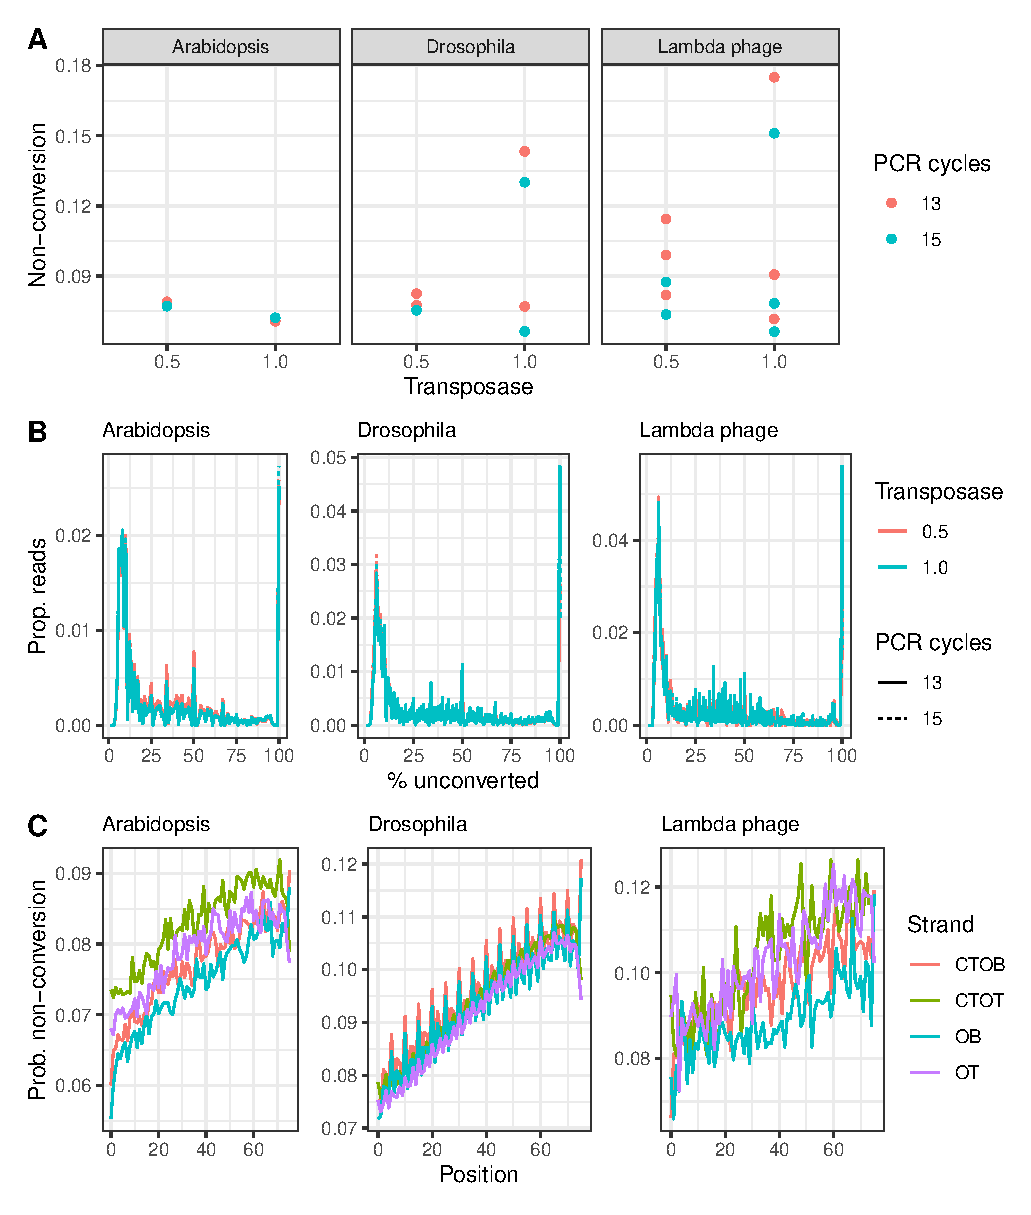
\includegraphics{figure1.eps}
    \caption{
        Cytosine non-conversion within and between reads on unmethylated DNA from \textit{A. thaliana}, the entire \textit{D. melanogaster} and Lambda phage. For \textit{A. thaliana}, data are shown for reads aligning to the first 75kb of chloroplast.
        (A) Overall cytosine non-conversion rates across for different ratios of Tn5 to DNA and number of PCR cycles performed.
        (B) The distribution of the proportion of unconverted cytosines across reads. For clarity, reads with no unconverted cytosines are not shown.
        (C) The probability of observing an unconverted cytosine across each read on the four strands generated by bisulphite libraries (OT=original top strand; OB=original bottom; CTOT=complementary to original top; CTOB=complementary to original bottom) averaged over libraries.
    }
    \label{fig:reads}

\end{figure}

We investigated how and where cytosine non-conversion errors occur in plant, fly and viral DNA.
We prepared bisulphite libraries for samples of the \textit{Arabidopsis thaliana} reference accession \textit{Columbia} (Col-0), \textit{Drosophila melanogaster} and the Lambda phage.
Plant chloroplasts, fruit flies and this virus lack cytosine methylation, so any unconverted cytosines we observe must be erroneous.
For \textit{Arabidopsis} we focussed on the first half of the chloroplast, beceuase the second half shows strong homology with one of the autosomes.
To identify possible technical artefacts we modified the strand-displacement protocol described by \textcite{weichenhan2018tagmentation} to use two concentrations of transposase, and either 13 or 15 PCR cycles.
Overall cytosine non-conversion rates were very high, ranging from a few percent up to more than 17\% (figure \ref{fig:reads}A).
There was substantial variation between libraries, but there was no consistent effect of species, transposase concentration or number of PCR cycles.
High non-conversion do not seem to be constrained to any species, and there is substantial stochasticity between samples.

To investigate the phenomenon further we examined the distribution of cytosines non-conversion within and between reads.
Reads containing at least one cytosine fell into three categores.
The majority of reads (mean=71\%) showed no unconverted cytosines at all.
Remaining reads were roughly evenly split between those where every cytosine on a read was unconverted, and those where a small proportion of cytosines were unconverted (figure \ref{fig:reads}B).
In the latter case, the peak matched the overall non-conversion rates (figure \ref{fig:reads}A).
This indicates that two distinct processes contribute to cytosines non-conversion.

We found that non-conversion errors were more likely to occur towards the 3` than the 5` end of the read (figure \ref{fig:reads}C).
This may be partly due to the general tendency of sequence quality to decline along a read.
However, this is unlikely to be the main cause in this case because Phred scores are consistently high across reads.
This pattern must be due to reads with only partial non-conversion, since fully unconverted reads would increase non-conversion uniformly across the whole read.

There is also some evidence that non-conversion errors depend on strand.
Bisulphite libraries typically distinguish between four strands: the original top and bottom strands (OT, OB), and the strands complementary to the original strands that are synthesised during PCR (complementary to original top (CTOT) and complementary to original bottom, (CTOB)).
In the \textit{Arabidopsis} and Lambda phage samples there is a slight tendency for the top strands to have increased errors than the bottom strands, and for the complementary strands to have increased errors compared to the corresponding original strands.
In the \textit{Drosophila} samples there also appears to be a periodicity in the probabilities of non-conversion every five bases on the OB and CTOB strands only.
The reasons for this potential strand specificity remain unclear.

In summary, these results indicate that non-conversion errors occur at high frequency in samples from diverse organisms. It appears that affected reads result from two distinct processes that generate completely and partially unconverted reads.

\subsection{Non-conversion errors vary across the genome}

\begin{figure}
    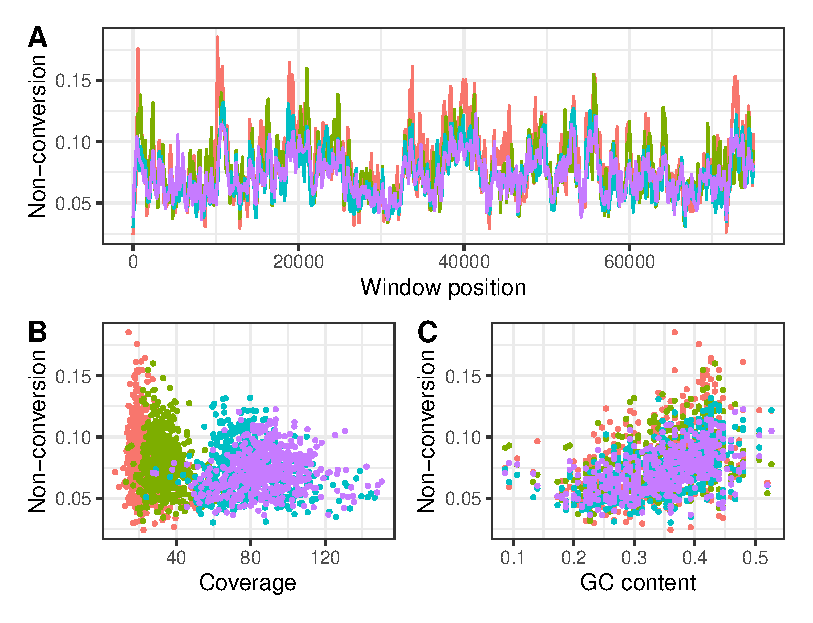
\includegraphics{figure2.eps}
    \caption{
        Variation in cytosine non-conversion across the first half of the chloroplast in four independent replicate library preparations of the \textit{Arabidopsis} accession Col-0.
        (A) 150bp windows across the chloroplast.
        (B) Across annotated features on the chloroplast.
        (C) Relationship between non-conversion and coverage per base.
        (D) Relationship between non-conversion and GC content.
    }
    \label{fig:uncertainty}
\end{figure}

Taking the average cytosine non-conversion rate on control DNA gives a point estimate of the genome-wide non-conversion rate, but this might mask variation in error rates between sites.
To investigate this we estimated non-conversion rates in 150bp windows across the \textit{Arabidopsis} chloroplast.
We found substantial variation in cytosine non-conversion across the \textit{Arabidopsis} chloroplast, in cases as much as five-fold between windows (figure \ref{fig:uncertainty}A).
One explanation for this is that there is much less data per window than for the whole chloroplast, so estimates at any individual window will have larger standard errors, inflating the variance between windows.
However, the observed variance between windows was 6.4-fold greater than between simulated draws from a binomial distribution using the observed coverage at each window as the number of trial and the global mean non-conversion rate as the mean (figure?).
Moreover, Spearman correlation coefficients ($\rho$) between replicates ranged from 0.71 to 0.84, showing that the pattern was remarkably consistent between technical replicates of the library preparation protocol.
This indicates that the variation in non-conversion across the chloroplast reflects something intrinsic about the DNA rather than stochastic variation.

What aspects of the DNA or data might explain this variation?
There was a weak negative correlation ($\rho$ between -0.29 and -0.10) between non-conversion and coverage at each window in three samples, with a weak positive correlation in the remaining sample ($\rho = 0.18$; figure \ref{fig:uncertainty}C).
Nevertheless, while very low coverage causes estimates to be noisy, the lowest coverage per cytosine in any window was 32.7x, so this cannot account for a large proportion of the variance.
There were also consistent positive correlations between non-conversion and GC content in each window across samples ($\rho$ between 0.43 and 0.55; figure \ref{fig:uncertainty}D).
Say something about what this means.
Add a conclusion sentence.

In summary, it appears that non-conversion errors vary between regions of the genome in a systematic way. Although the underlying reasons for this are unclear, this observation warrant caution in using a single point estimate to account for errors across the genome.

\subsection{Methylation estimates depend more on sample size than non-conversion errors}

fig:
    deterministic error rates
    simulation, showing data without errors, data with known errors, data with best guess, estimate accounting for uncertainty
    Plot variance for ibid as a function of coverage


Estimating mean methylation is a binomial process
We can account for errors by allowing observed state of methylated and unmethylated reads to be correct or incorrect.
We model the probability that (1) truly unmethylated cytosines appear methylated (false non-conversion) or (2) truly methylated cytosines appear unmethylated (false converion; see Materials and Methods for full details).
These sources of error have the strongest effects when mean methylation is close to zero and one respectively (figure \ref{fig:}).
The true mean methylation level accounting for these error rates can then be estimated algebraicly (see Materials and Methods).
Can also estimate it accounting for uncertainty in theta.

To investigate how this works we simulated data.
We simulated loci of 250 cytosines, corresponding to TE's of 1000 bp, because the mean is 798.
Mean methylation of 0.15, because this is realistic for TEs and fairly close to the error distribution.
At each locus we drew and error rate from a Beta
We also summed loci
This gives biologically realistic data

When error rates are known we can correct for them as well as if there were no errors.
When errors are not know there is more error
May or may not be more when we integrate.
However, binomial sampling is huge
For small samples variance between estimates is massive even for perfect data
Statement about change in variance.
Summing over loci works
You need to some over about 100 TEs
As long as you sum enough, conversion errors don't matter.

\subsection{Reliable imputation of methylation state}

Fig: Three panels showing calls on chloroplast, TEs and genes.

Differences in methylation are often due to the effects distinct biological pathways
For example, Zhang et al split genes into unmethylated 
In this case it makes more sense to describe the state
For example, Zhang et al. distinguish unmethylated, CG- and TE-like methylation

Gaut and pals do something, but it's not ideal
We can do better by modelling the probability that methylation in each context
comes from the error process, or from an alternative process with more methylation
than that.



\section{Discussion}


What could explain this?
Reads not being trimmed correctly, or poor conversion.
We address this, but it's unlikely because these are the same between protocols
More likely to be to do with the strand displacement/gap repair step, which differ between protocols
dNTPS with mC are being incorporated, for example via repair of single-strand nicks.
PCR bias?


Discuss \cite{lu2015improved} and \cite{suzuki2018whole}'s solution's to the problem

\section{Materials and Methods}

\subsection{Biological material}

\subsection{Statistical models to accounts for conversion errors}

\subsubsection{Error rates in a binomial model}

Methylation pipelines tell us that of a total of $n$ reads mapping to a region of a genome, we observe $y$ reads mapping to methylated cytosines and $n-y$ reads mapping to unmethylated cytosines. The goal is to estimate the true mean methylation level $\theta$ which generated these data, accounting for conversion errors.

In the absence of errors, the likelihood of the data given $\theta$ is binomially distributed as
\begin{equation}
    \label{eqn:classic-binomial}
    \Pr(y| \theta) = {n \choose y} \theta^y(1-\theta)^{n-y}
\end{equation}
with mean $\theta=y/n$.
Data are not perfect, so we would like to incorporate two error terms:
\begin{itemize}
    \item $\lambda_1$ is the probability that an unmethylated cytosine appears methylated (the bisulphite non-conversion rate).
    \item $\lambda_2$ is the probability that a methylated cytosine appears unmethylated.
\end{itemize}
Cytosines observed to be methylated may thus be either truly methylated with probability $\theta(1-\lambda_2)$ or truly unmethylated with probability $(1-\theta)\lambda_1$. Likewise, a cytosine observed to be unmethylated may be either truly unmethylated with probability $(1-\theta)(1-\lambda_1)$ or truly methylated with probability $\theta \lambda_2$.
This changes the likelihood to
\begin{equation}
    \label{eqn:binom-with-errors}
    \Pr(y | \theta, \lambda_1, \lambda_2) = 
    {n \choose y}
    [\theta(1-\lambda_2) + (1-\theta)\lambda_1]^y
    [\theta \lambda_2 + (1-\theta)(1-\lambda_1)]^{n-y}
\end{equation}
Summarising $p=[\theta(1-\lambda_2) + (1-\theta)\lambda_1]$ for brevity, this has a closed-form maximum-likelihood estimate
\begin{equation}
    \label{eqn:ml-theta}
    \hat{\theta} = \frac{\lambda_1-p}{\lambda_1 + \lambda_2 -1}
\end{equation}

\subsubsection{Uncertainty in error rates}

The above formulation is valid for the case where there is a clear point estimate for error rates.
If there is substantial uncertainty around these estimates values, and especially if they are likely to vary across the genomes, then the $\theta$ and error rates can be modelled as coming from Beta distributions with shape parameters $a$ and $b$:
\begin{equation}
    \theta \sim \textrm{Beta}(a_{\theta}, b_{\theta})
\end{equation}
\begin{equation}
    \lambda_1 \sim \textrm{Beta}(a_{\lambda_1}, b_{\lambda_1})
\end{equation}
\begin{equation}
    \lambda_2 \sim \textrm{Beta}(a_{\lambda_2}, b_{\lambda_2})
\end{equation}
The distributions over $\Pr(\theta)$, $\Pr(\lambda_1)$ and $\Pr(\lambda_2)$ represent prior distributions of $\theta$ and error rates, and can be estimated from other data.
For example, $\lambda_1$ can be estimated by counting the proportion of all unconverted cytosines in windows of DNA that is known to be unmethylated to get a distribution of error rates, and taking mean $\bar{x}$ and variance $\sigma^2_x$ of these estimates.
The shape parameters of the Beta distribution for $\Pr(\lambda_1)$ can be calculated by method-of-moments as
\begin{equation}
    \hat{a}_{\lambda_1} = \bar{x}(\frac{\bar{x}(1-\bar{x})}{\sigma^2_x}-1)
\end{equation}
\begin{equation}
    \hat{b}_{\lambda_1} = 1-\bar{x}(\frac{\bar{x}(1-\bar{x})}{\sigma^2_x}-1) 
\end{equation}

We can use this information to estimate $\theta$ by integrating out values for error rates.
The joint posterior distribution of $\theta, \lambda_1, \lambda_2$ is then
\begin{equation}
    \Pr(\theta, \lambda_1, \lambda_2 | y, \pi)
    \propto 
    \Pr(y | \theta, \lambda_1, \lambda_2)
    \Pr(\theta | a_{\theta}, b_{\theta})
    \Pr(\lambda_1 | a_{\lambda_1}, b_{\lambda_1})
    \Pr(\lambda_2 | a_{\lambda_2}, b_{\lambda_2})
\end{equation}
where $\pi=\{a_{\theta}, a_{\lambda_1}, a_{\lambda_2}, b_{\theta}, b_{\lambda_1}, b_{\lambda_2}\}$ for brevity.
The marginal posterior distribution for $\theta$ can be found by integrating over $\Pr(\lambda_1)$ and $\Pr(\lambda_2)$.
The posterior mean of this distribution is the most probable value of $\theta$ accounting for all possible values of error rates. It ought to be possible to get a closed-form point estimate by setting the first derivative to zero and solving for $\theta$, but I haven't work out how yet.

\subsubsection{Methylation status}

In some cases it may be advantageous to think of DNA methylation as being in particular discrete states.
For example, [Zhang et al. (2020)](https://www.pnas.org/doi/full/10.1073/pnas.1918172117) present a case that DNA methylation (at least on genes) represents a continuum between unmethylated DNA, TE-like methylation (CG, CHG and CHH methylation), and CG-only methylation.
In this case it is likely that these states represent the effects of distinct biological pathways, so makes more sense to identify discrete states than to make quantitative estimates of methylation.
We would thus like to partition the genome into regions that look like each of these contexts.

Given total numbers of apparently methylated and unmethylated reads at each site ($y_{CG}$, $y_{CHG}$ and $y_{CHH}$) and reasonable point estimates of $\lambda_1$ and $\lambda_2$ we can use the estimate of $\hat{\theta}$ from \ref{eqn:ml-theta} above to calculate likelihoods that a window is unmethylated ($L_U$), TE-like methylated ($L_{TEm}$), or CG-methylated ($L_{CG}$):
\begin{equation}
    \label{eqn:lik-unmethylated}
    L_{U} = 
    \Pr( y_{CG} | \theta_{CG} =0, \lambda_1, \lambda_2)
    \Pr(y_{CHG} | \theta_{CHG}=0, \lambda_1, \lambda_2)
    \Pr(y_{CHH} | \theta_{CHH}=0, \lambda_1, \lambda_2)
\end{equation}
\begin{equation}
    \label{eqn:lik-mCG}
    L_{CG} = 
    \Pr( y_{CG} | \theta_{CG}>0, \lambda_1, \lambda_2)
    \Pr(y_{CHG} | \theta_{CHG}=0, \lambda_1, \lambda_2)
    \Pr(y_{CHH} | \theta_{CHH}=0, \lambda_1, \lambda_2)
\end{equation}
\begin{equation}
    \label{eqn:lik-TEm}
    L_{TEm} = 
    \Pr( y_{CG} | \theta_{CG}>0, \lambda_1, \lambda_2)
    \Pr(y_{CHG} | \theta_{CHG}>0, \lambda_1, \lambda_2)
    \Pr(y_{CHH} | \theta_{CHH}>0, \lambda_1, \lambda_2)
\end{equation}

This assumes errors are the same for CG, CHG and CHH sites; this is reasonable because we think errors happen in a tube, not a cell. It is probably sensible to set a minimum bound on the number of CG sites in a window such that you could actually expect to distinguish $\theta_{CG}$ and error rates.

One could just take the model with the highest likelihood (better: AIC), and that may well be enough for our purposes. To perform formal likelihood ratio tests we first note that $L_{CG}$ is nested within $L_{TEm}$ and $L_{U}$ is nested within $L_{CG}$. Likelihood ratio tests can then be performed assuming the test statistic under the null is $\chi^2$-distributed 
with 1 degree of freedom.



We can likewise modify the likelihood calculations of methylation statuses to include distributions of error rates.
In this case we define distinct prior distributions for the expected distribution of true methylation under different scenarios, and calculate the support for each.
For example, it is reasonable to expect that unmethylated DNA has a true methylation rate very close to zero, and hence we might define parameters for $\Pr(\theta)$ that give values very small means.

\section{Ackowledgements}

We thank Robert Schmitz, Dieter Weichenhan and members of the Nordborg group for discussion of the results.
We specifically thank Yoav Voichek for technical assistance on how to disembowel SAM files.

\printbibliography %Prints bibliography

\end{document}